\documentclass{article}



\usepackage{fullpage}
\usepackage{nopageno}
\usepackage{amsmath}
\usepackage{amsfonts}
\usepackage{graphicx}
\usepackage{framed}
\usepackage{xcolor}

\definecolor{dark_red}{rgb}{0.5,0.0,0.0}
\definecolor{dark_green}{rgb}{0.0,0.5,0.0}
\definecolor{dark_blue}{rgb}{0.0,0.0,0.5}

\newcommand{\dr}[1]{\textcolor{dark_red}{#1}}
\newcommand{\dg}[1]{\textcolor{dark_green}{#1}}
\newcommand{\db}[1]{\textcolor{dark_blue}{#1}}


\begin{document}

\begin{tabular}{cc}
\parbox{0.5\textwidth}{
In the image on the right, a gear of radius \(R\) is rotating counterclockwise at an angular speed of \(\omega\). After a time interval of \(\Delta t\), the gear has turned by \(\omega \Delta t\). The rim of the gear is moving at a speed of \(v\). After the same time interval of \(\Delta t\), the rim of the gear has moved a distance of \(v\Delta t\). The distance that the gear rim has moved can also be computed from the rotated angle of \(\omega \Delta t\) and the gear's radius \(R\): \(R \cdot \omega \Delta t\). This gives the relationship \(v \Delta t = R \omega \Delta t\) which is equivalent to:
\[v = R \omega\]
} & \parbox{0.5\textwidth}{
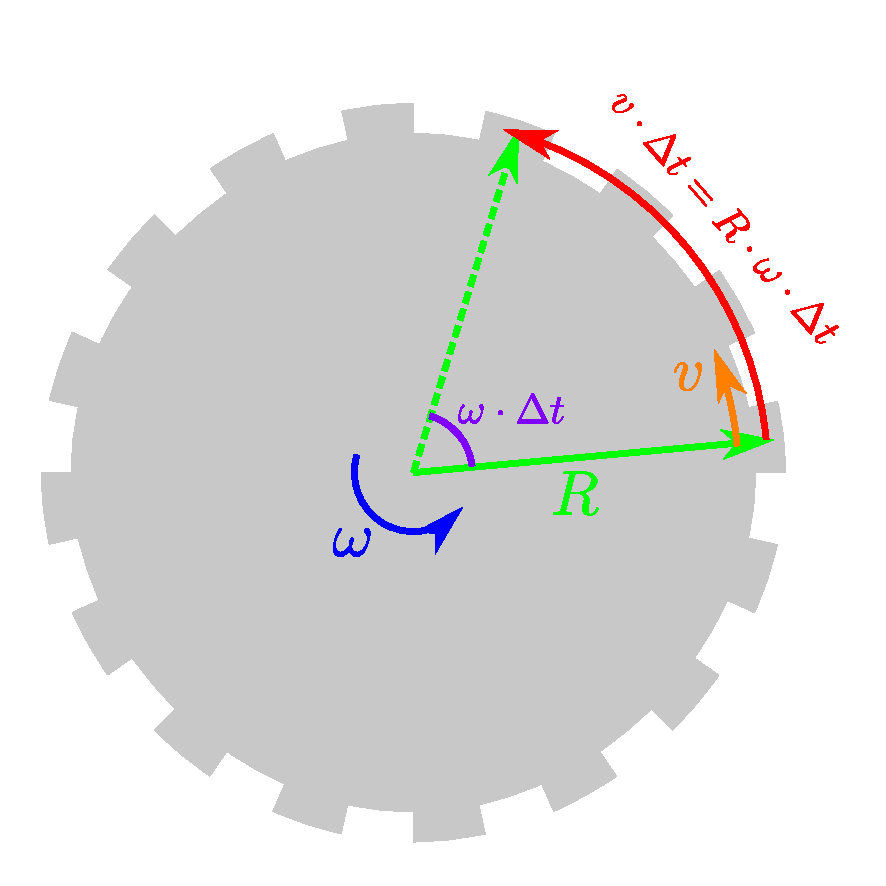
\includegraphics[width = 0.5\textwidth]{spinning_gear}
}
\end{tabular}

If a gear has a radius of \(R = 7\text{cm} = 0.07\text{m}\), and rotates once every \(T = 2\text{s}\), then with a full rotation of \(2\pi\) every time interval of \(T\), the angular speed is \(\omega = \frac{2\pi}{T} \approx 3.142 \text{s}^{-1}\). The speed of the rim is \(v = R\omega = 0.2199\text{m/s} = 21.99\text{cm/s}\).

Reasoning in the other direction, if the rim speed is now \(v = 30\text{cm/s} = 0.3000 \text{m/s}\) and the radius is unchanged, then the angular speed satisfies \(v = R\omega \iff \omega = \frac{v}{R} \approx 4.286 \text{s}^{-1}\). The time \(T\) required for a full revolution is: \(T = \frac{2\pi}{\omega} \approx 1.466 \text{s}\)

\end{document}


